\documentclass[a4paper,12pt]{article}

\usepackage{graphicx}
\usepackage{caption}
\usepackage{subcaption}
\usepackage{tikz}
\usepackage{pgf}
\usepackage{amsmath}
\usepackage{amssymb}
\usetikzlibrary{arrows.meta}
\usepackage[utf8]{inputenc}
\usepackage[english,greek]{babel}
\usepackage{hyperref}

\title{Προσομοίωση και Μοντελοποίηση \newline Δυναμικών Συστημάτων \newline 
\selectlanguage{english}Project\selectlanguage{greek}}
\author{Ρουσομάνης Γεώργιος (ΑΕΜ: 10703)}
\date{Ιούνιος 2025}

\begin{document}

\maketitle

\section*{Εισαγωγή}

\section*{Θέμα 1}

Σε αυτό το μέρος μελετάται ένα γραμμικό δυναμικό σύστημα δεύτερης τάξης της μορφής:
\begin{equation}
\dot{\mathbf{x}}(t) = \mathbf{A} \mathbf{x}(t) + \mathbf{B} u(t),
\label{eq:state_space_form}
\end{equation}
όπου $\mathbf{x}(t) \in \mathbb{R}^2$ είναι το διάνυσμα των καταστάσεων, και $u(t) \in \mathbb{R}$ 
η είσοδος του συστήματος. Οι πίνακες $\mathbf{A} \in \mathbb{R}^{2 \times 2}$ και 
$\mathbf{B} \in \mathbb{R}^{2 \times 1}$ είναι άγνωστοι αλλά σταθεροί. Επίσης, γνωρίζουμε ότι:
\begin{equation}
-3 \leq a_{11} \leq -1, \quad \quad b_2 \geq 1.
\label{eq:restrictions}
\end{equation}

Σκοπός είναι η ανάπτυξη και ανάλυση ενός αλγορίθμου πραγματικού χρόνου για την εκτίμηση  
$\hat{\mathbf{A}},\,\hat{\mathbf{B}}$ των πινάκων $A$ και $B$, με δεδομένο ότι τόσο η είσοδος 
$u(t)$ όσο και το διάνυσμα καταστάσεων $\mathbf{x}(t)$ είναι μετρήσιμα. Για τη σχεδίαση του 
αλγορίθμου, αρχικά υποθέτουμε ότι δεν υπάρχουν διαταραχές στις μετρήσεις των καταστάσεων του 
συστήματος. Στη συνέχεια, εισάγεται στο σύστημα σφάλμα πόλωσης και επανασχεδιάζεται ο αλγόριθμος, 
με στόχο τη μελέτη της επίδρασης του σφάλματος στην ακρίβεια των εκτιμήσεων. Για σκοπούς 
προσομοίωσης, χρησιμοποιούνται ως πραγματικές τιμές οι παρακάτω πίνακες:
\[
\mathbf{A} = 
\begin{bmatrix}
-2.15 & 0.25 \\
-0.75 & -2
\end{bmatrix}, \quad
\mathbf{B} = 
\begin{bmatrix}
0 \\
1.5
\end{bmatrix}.
\]

\subsection*{Εκτίμηση Παραμέτρων χωρίς Σφάλμα Πόλωσης}

Πρωτού προχωρήσουμε στη σχεδίαση του αλγορίθμου πραγματικού χρόνου για την εκτίμηση των 
$\mathbf{A}, \, \mathbf{B}$, πρέπει να επιλέξουμε το είδος της εισόδου που θα εφαρμόσουμε 
στο σύστημα, καθώς και τη συχνότητα δειγματοληψίας. Μία συνήθης πρακτική για την επιλογή της 
συχνότητας δειγματοληψίας είναι να την ορίζουμε περίπου δέκα φορές μεγαλύτερη από το εύρος 
ζώνης του συστήματος. Ωστόσο, επειδή το μοντέλο μας υπάγεται στην κατηγορία ``γκρι κουτί'', 
η εκ των προτέρων γνώση μας για το σύστημα δεν επαρκεί για τον άμεσο υπολογισμό του εύρους ζώνης.

\subsubsection*{Επιλογή συχνότητας δειγματολειψίας}

Εφαρμόζουμε βηματική είσοδο στο σύστημα ώστε να εκτιμήσουμε την κυρίαρχη σταθερά χρόνου  
και να αποκτήσουμε μία πρώτη εικόνα για τη δυναμική του. Η βηματική απόκριση του συστήματος  
παρουσιάζεται στο Σχήμα~\ref{fig:task1_step_response} για συχνότητα δειγματοληψίας $f_s = 1$
\selectlanguage{english}kHz\selectlanguage{greek}. Η $f_s$ επιλέχθηκε αυθαίρετα ως μία υψηλή τιμή, 
επαρκής για να αποτυπώσει τη δυναμική του συστήματος.

Από το σχήμα είναι εμφανές ότι η απόκριση της κατάστασης $x_2(t)$ είναι ταχύτερη αυτής της $x_1(t)$,
συνεπώς η σταθερά χρόνου του συστήματος θα προσδιοριστεί μέσω της $x_2(t)$. Στην απόκριση της
$x_2(t)$ δεν παρατηρείται υπερύψωση, άρα ο χρόνος αποκατάστασης $t_s$ ορίζεται ως ο χρόνος που απαιτείται
ώστε το σύστημα να φτάσει στο $98\%$ της εξόδου του. Από το σχήμα βλέπουμε ότι $t_s \approx 2$
\selectlanguage{english}sec\selectlanguage{greek}. Η σταθερά χρόνου είναι $\tau \approx t_s / 4 = 0.5$
\selectlanguage{english}sec\selectlanguage{greek}. Συνεπώς, η συχνότητα δειγματολειψίας πρέπει να 
ικανοποιεί $f_s > 10 / \tau = 20$\selectlanguage{english}Hz\selectlanguage{greek}.

Για το πραγματικό σύστημα, οι ιδιοτιμές του πίνακα $\mathbf{A}$ είναι $\lambda_{1,2} = -2.075 \pm 0.4265j$, 
και η σταθερά χρόνου $\tau = \frac{1}{\zeta \omega_n} = 0.482$, η οποία είναι πολύ κοντά στην αρχική 
μας εκτίμηση.

\begin{figure}[htbp]
  \centering
  \begin{subfigure}[b]{0.45\textwidth}
    \centering
    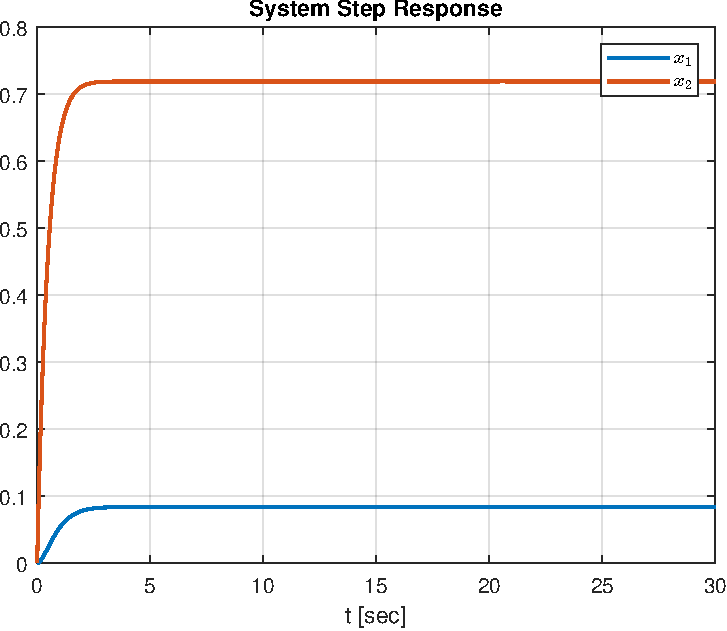
\includegraphics[width=\textwidth]{plot/task1_step_response.pdf}
    \caption{}
    \label{fig:task1_step_response}
  \end{subfigure}
  \hfill
  \begin{subfigure}[b]{0.45\textwidth}
    \centering
    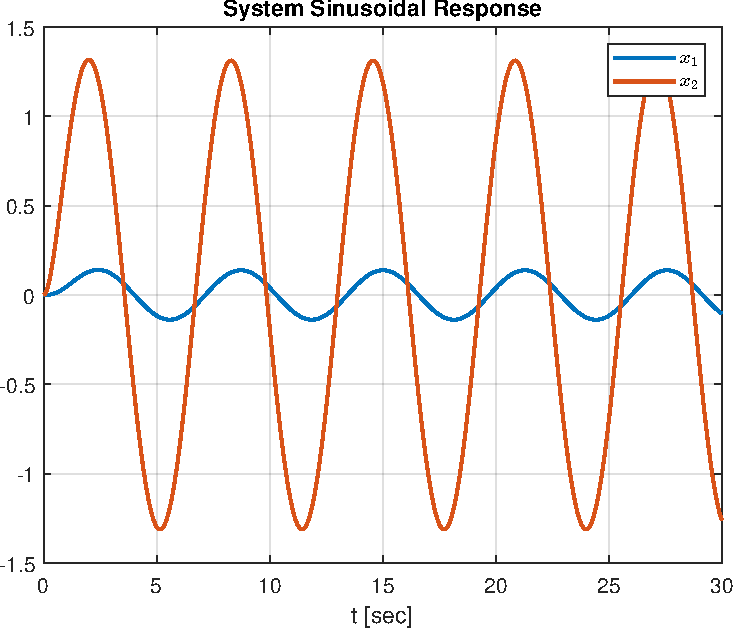
\includegraphics[width=\textwidth]{plot/task1_sinusoidal_response.pdf}
    \caption{}
    \label{fig:task1_sinusoidal_response}
  \end{subfigure}
  \caption{Απόκριση του συστήματος για α) βηματική είσοδο, β) $u(t) = 2 \sin t$}
  \label{fig:task1_response}
\end{figure}

\subsubsection*{Επιλογή εισόδου}

Για να αποτυπωθεί πλήρως η δυναμική του συστήματος, είναι σημαντικό η είσοδος να περιέχει αρκετές
συχνότητες ώστε να διεγείρει όλους τους ρυθμούς του συστήματος. Επίσης, με κατάλληλη επιλογή της
εισόδου ώστε να ικανοποιεί την Συνθήκη Εναπομείνουσας Διέγερσης (ΣΕΔ), οι μέθοδοι εκτίμησης παραμέτρων 
πραγματικού χρόνου (κλίσης, \selectlanguage{english}Lyapunov\selectlanguage{greek}) μας εγγυόνται την 
σύγκλιση των παραμετρικών σφαλμάτων στο μηδέν.

Το γραμμικό μας σύστημα είναι τάξεως $n=2$. Για να ικανοποιεί η είσοδός μας $u$ μία ΣΕΔ πρέπει
να περιέχει τουλάχιστον $m = \left\lceil \frac{n}{2} \right\rceil$ διακριτές συχνότητες και τότε
το σήμα $u$ λέγεται επιμένουσα διέγερση τάξεως $n$. Στην ανάλυσή μας παρακάτω χρησιμοποιούμε ως είσοδο
την $u(t) = 2 \sin t$.

\subsubsection*{Μέθοδος \selectlanguage{english}Lyapunov\selectlanguage{greek} με προβολή}
Λόγω της εκ των προτέρων γνώσης που έχουμε για το επιτρεπτό εύρος τιμών ορισμένων παραμέτρων, 
ο χώρος αναζήτησης $\Theta$ των παραμέτρων του μοντέλου θα περιορίζεται σε ένα υποσύνολο του $\mathbb{R}^n$.
Θα χρησιμοποιήσουμε κάποιο αναδρομικό αλγόριθμο προβολής ο οποίος εξασφαλίζει ότι οι εκτιμήσεις των
παραμέτρων παραμένουν εντός του $\Theta$. Ειδικότερα θα χρησιμοποιήσουμε τη μέθοδο 
\selectlanguage{english}Lyapunov\selectlanguage{greek} με προβολή.

Πρωτού προχωρήσουμε στην εκτίμηση των παραμέτρων, θα εξετάσουμε την ευστάθεια της μεθόδου 
\selectlanguage{english}Lyapunov\selectlanguage{greek} με Μ-δομή χωρίς περιορισμούς.

Το σύστημα αναγνώρισης είναι:
\begin{equation}
    \dot{\hat{\mathbf{x}}} = \hat{\mathbf{A}}\mathbf{x} + \hat{\mathbf{B}} u + 
    \mathbf{C}(\mathbf{x} - \hat{\mathbf{x}}),
    \label{eq:lyapunov_mixed_identification_system}
\end{equation}
όπου $\mathbf{C}$ συμμετρικός και θετικά ημιορισμένος πίνακας. Η παράγωγος του σφάλματος αναγνώρισης 
$\mathbf{e} = \mathbf{x} - \hat{\mathbf{x}}$ 
βρίσκεται:
\begin{equation}
    \dot{\mathbf{e}} = -\tilde{\mathbf{A}}\mathbf{x} - \tilde{\mathbf{B}}u - \mathbf{C}\mathbf{e}
    \label{eq:lyapunov_mixed_identification_error_derivative}
\end{equation}
όπου $\tilde{\mathbf{A}} = \hat{\mathbf{A}} - \mathbf{A}$,
$\tilde{\mathbf{B}} = \hat{\mathbf{B}} - \mathbf{B}$ τα παραμετρικά σφάλματα.
Ως συνάρτηση \selectlanguage{english}Lyapunov\selectlanguage{greek} επιλέγεται η:
\begin{equation}
    V = \frac{1}{2}\mathbf{e}^{\top}\mathbf{e} + 
    \frac{1}{2}\mathrm{Tr}\{\tilde{\mathbf{A}}^{\top}\tilde{\mathbf{A}}\}
    + \frac{1}{2}\mathrm{Tr}\{\tilde{\mathbf{B}}^{\top}\tilde{\mathbf{B}}\}
    \label{eq:lyapunov_function}
\end{equation}
Παραγωγίζοντας την (\ref{eq:lyapunov_function}) και αντικαθιστώντας
την (\ref{eq:lyapunov_mixed_identification_error_derivative}) προκύπτει:
\begin{equation}
    \dot{V} = -\mathbf{e}^{\top}\mathbf{C}\mathbf{e} + 
    \mathrm{Tr}\{\tilde{\mathbf{A}}^{\top}\dot{\hat{\mathbf{A}}} + 
    \tilde{\mathbf{B}}^{\top}\dot{\hat{\mathbf{B}}} - 
    \tilde{\mathbf{A}}\mathbf{x}\mathbf{e}^{\top} - 
    \tilde{\mathbf{B}}u\mathbf{e}^{\top}\}.
    \label{eq:lyapunov_mixed_function_derivative_1}  
\end{equation}
Επιλέγουμε:
\begin{equation}
    \begin{aligned}
        \dot{\hat{\mathbf{A}}} = \mathbf{e}\mathbf{x}^{\top} \\ 
        \dot{\hat{\mathbf{B}}} = \mathbf{e}u^{\top}
    \end{aligned}
    \label{eq:lyapunov_mixed_update_formula}
\end{equation}
και η (\ref{eq:lyapunov_mixed_function_derivative_1}) γίνεται:
\begin{equation}
    \dot{V} = -\mathbf{e}^{\top}\mathbf{C}\mathbf{e}
    \label{eq:lyapunov_mixed_function_derivative_2}
\end{equation}
Βλέπουμε ότι στη μικτή δομή ισχύει $\dot{V} \leq 0, \, \forall t$, καθώς ο $\mathbf{C}$ είναι 
συμμετρικός και θετικά ημιορισμένος. Συνεπώς, το σύστημα (\ref{eq:lyapunov_mixed_identification_system}), 
(\ref{eq:lyapunov_mixed_update_formula}) είναι ευσταθές.

Στην ανάλυσή μας θέσαμε $\mathbf{C} = k \mathbf{I}$, όπου $\mathbf{I}$ είναι ο μοναδιαίος πίνακας και 
$k > 0$ το κέρδος. Η επιλογή του $k$ έγινε με τη μέθοδο 
\selectlanguage{english}trial and error\selectlanguage{greek}. Μεγαλύτερες τιμές του $k$ έχουν ως 
αποτέλεσμα να υπερισχύει ο διορθωτικός όρος $\mathbf{C}(\mathbf{x} - \hat{\mathbf{x}})$ στην 
(\ref{eq:lyapunov_mixed_identification_system}), οδηγώντας σε ταχύτερη σύγκλιση. Ωστόσο, πολύ μεγάλες 
τιμές του $k$ ενδέχεται να καταστήσουν το σύστημα άκαμπτο. Τελικά, επιλέγουμε $k = 1$.

Έχοντας εξασφαλίσει την ευστάθεια του αλγορίθμου απουσία περιορισμών, συνεχίζουμε με την σχεδίαση του
αναδρομικού αλγορίθμου προβολής. Έστω
\[
\hat{\theta} =
\begin{bmatrix}
    \hat{\alpha}_{11} & \hat{\alpha}_{12} & \hat{\alpha}_{21} & \hat{\alpha}_{22} & \hat{b}_1 & \hat{b}_2
\end{bmatrix}^{\top}
\]
το διάνυσμα των εκτιμήσεων των παραμέτρων που προκύπτει από το σύστημα (\ref{eq:lyapunov_mixed_identification_system}), (\ref{eq:lyapunov_mixed_update_formula}). 
Θέλουμε να εξασφαλίσουμε ότι το $\hat{\theta}$ θα παίρνει τιμές εντός του κυρτού συνόλου:
\[
\Theta = \{\hat{\theta} \in \mathbb{R}^6:\, g(\hat{\theta}) \leq 0\}
\]
όπου η $g(\hat{\theta}) \in \mathbb{R}^3$ έχει διάσταση όση και το πλήθος των περιορισμών.
Από την (\ref{eq:restrictions}) έχουμε:
\[
\begin{aligned}
    \alpha_{11} \ge -3 \Rightarrow - \alpha_{11} - 3 \le 0 \\
    \alpha_{11} \le -1 \Rightarrow \alpha_{11} + 1 \le 0 \\
    b_2 \ge 1 \Rightarrow 1 - b_2 \le 0
\end{aligned}
\]
Συνεπώς η $g(\hat{\theta})$ θα είναι:
\[
    g(\hat{\theta}) = 
    \begin{bmatrix}
        - \alpha_{11} - 3 \\
        \alpha_{11} + 1 \\
        1 - b_2
    \end{bmatrix}
\]
και η Ιακωβιανή της $g(\hat{\theta})$:
\[
    \mathbf{J}_g(\hat{\theta}) = 
    \begin{bmatrix}
         \nabla g_1(\hat{\theta}) \\
         \nabla g_2(\hat{\theta}) \\
         \nabla g_3(\hat{\theta})
    \end{bmatrix} = 
    \begin{bmatrix}
        -1 & 0 & 0 & 0 & 0 & 0 \\
        1 & 0 & 0 & 0 & 0 & 0 \\
        0 & 0 & 0 & 0 & 0 & -1
    \end{bmatrix}
\]
Ο αλγόριθμος \selectlanguage{english}Lyapunov\selectlanguage{greek} με προβολή μεικτής δομής που πετυχαίνει
το παραπάνω αποτέλεσμα είναι:
\begin{equation}
    \dot{\hat{\theta}}_\Pi = 
    \begin{cases}
    \dot{\hat{\theta}}, & \text{αν } g_i(\hat{\theta}) < 0 
    \text{ ή } \nabla g_i^\top \dot{\hat{\theta}} \leq 0 \\
    \dot{\hat{\theta}} - 
    \mathbf{\Gamma} \frac{\nabla g_i {\nabla g_i}^{\top}}{{\nabla g_i}^{\top} \mathbf{\Gamma} \nabla g_i}
    \dot{\hat{\theta}}, & \text{διαφορετικά}
    \end{cases}
    \label{eq:lyapunov_mixed_projection}
\end{equation}
όπου $\mathbf{\Gamma}  = \mathbf{\Gamma}^{\top} \in \mathbb{R}^{6 \times 6}$ ο πίνακας κέρδους προσαρμογής
και ο δείκτης $i$ υποδηλώνει τον $i$-οστό περιορισμό. Ο διορθωτικός όρος 
$- \Gamma \nabla g_i \left( \nabla g_i^\top \Gamma \nabla g_i \right)^{-1} \nabla g_i^\top 
\dot{\hat{\theta}}$ εγγυάται ότι $\hat{\theta} \in \Theta, \, \forall t \ge 0$ με την προϋπόθεση ότι
$\hat{\theta}(0) \in \Theta$. Πράγματι:
\[
\begin{aligned}
\dot{\hat{\theta}}_{\Pi}^{\top} \nabla g_i &= \dot{\hat{\theta}}^{\top} \nabla g_i - 
\dot{\hat{\theta}}^{\top} \frac{\nabla g_i \nabla g_i^{\top}}{\nabla g_i^{\top} \mathbf{\Gamma} \nabla g_i}
\mathbf{\Gamma}^{\top} \nabla g_i \\
&= \dot{\hat{\theta}}^{\top} \nabla g_i - \dot{\hat{\theta}}^{\top} \nabla g_i 
\frac{\nabla g_i^{\top} \mathbf{\Gamma} \nabla g_i}{\nabla g_i^{\top} \mathbf{\Gamma} \nabla g_i} \\
&= 0
\end{aligned}
\]
Συνεπώς, όταν ο $i$-οστός περιορισμός είναι ενεργός, η γωνία μεταξύ των $\dot{\hat{\theta}}_{\Pi}^{\top}$
και $\nabla g_i$ είναι ορθή, άρα η νέα εκτίμηση $\hat{\theta}$ θα κινηθεί εφαπτομενικά πάνω στο σύνορο του 
$\Theta$.

Η ανάλυση της ευστάθειας που προηγήθηκε, αφορούσε τη μέθοδο 
\selectlanguage{english}Lyapunov\selectlanguage{greek} μεικτής δομής απουσία περιορισμών. Αποδεικνύεται 
ότι η προσθήκη του διορθωτικού όρου στην (\ref{eq:lyapunov_mixed_projection}) όχι μόνο δεν επηρεάζει 
αρνητικά την ευστάθεια του συστήματος, αλλά αντιθέτως καθιστά την παράγωγο της συνάρτησης 
\selectlanguage{english}Lyapunov\selectlanguage{greek} πιο αρνητική. Συνεπώς, τα συμπεράσματά μας περί
ευστάθειας μεταφέρονται αυτούσια και στην περίπτωση παρουσίας περιορισμών.

Αν για την εκτίμηση των παραμέτρων επιλέγαμε την Π-δομή, το σύστημα αναγνώρισης θα ήταν
\[
    \dot{\hat{\mathbf{x}}} = \hat{\mathbf{A}}\hat{\mathbf{x}} + \hat{\mathbf{B}} u
\]
Ακολουθώντας την ίδια μεθοδολογία όπως και για την Μ-δομή, καταλήγουμε στην σχέση:
\[
\dot{V} = -\mathbf{e}^{\top}\mathbf{Α}\mathbf{e} 
\]
Για να είναι $\dot{V} \leq 0$, πρέπει ο πίνακας $\mathbf{A}$ να είναι συμμετρικός και θετικά ημιορισμένος,
κάτι το οποίο δεν ισχύει. Συνεπώς, όταν η συνάρτηση \selectlanguage{english}Lyapunov\selectlanguage{greek}
δίνεται από την (\ref{eq:lyapunov_function}), δεν μπορούμε να αποδείξουμε την ευστάθεια της μεθόδου 
\selectlanguage{english}Lyapunov\selectlanguage{greek} Μ-δομής.

Στο Σχήμα~\ref{fig:task1_lyapunov} φαίνεται η γραφική παράσταση της συνάρτησης 
\selectlanguage{english}Lyapunov\selectlanguage{greek} καθώς και της παραγώγου της, για βηματική είσοδο 
(αριστερά) και ημιτονοειδή είσοδο $u(t) = 2 \sin t$ (δεξιά). Παρατηρούμε ότι και στις δύο περιπτώσεις 
ισχύει $V \geq 0, \, \dot{V} \leq 0, \forall t$, γεγονός που επιβεβαιώνει την ευστάθεια του συστήματος 
εκτίμησης παραμέτρων.

\begin{figure}[htbp]
  \centering
  \begin{subfigure}[b]{0.45\textwidth}
    \centering
    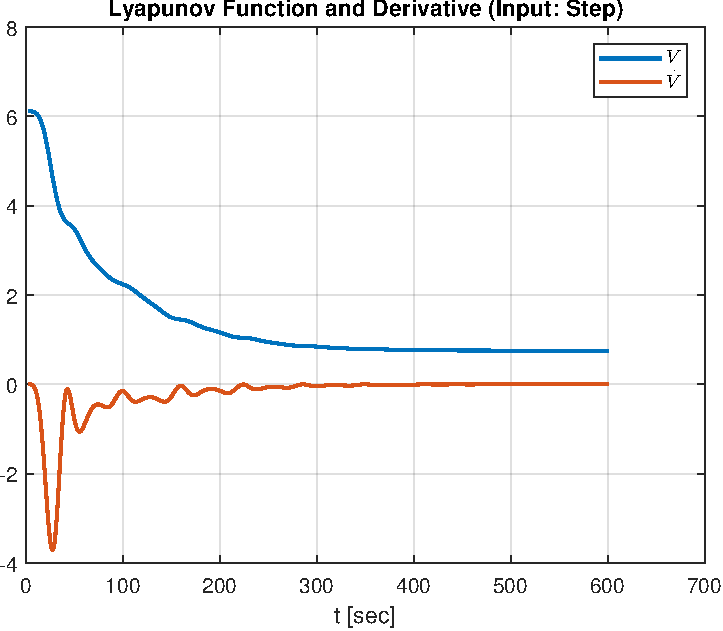
\includegraphics[width=\textwidth]{plot/task1_lyapunov_step.pdf}
    \caption{}
    \label{fig:task1_lyapunov_step}
  \end{subfigure}
  \hfill
  \begin{subfigure}[b]{0.45\textwidth}
    \centering
    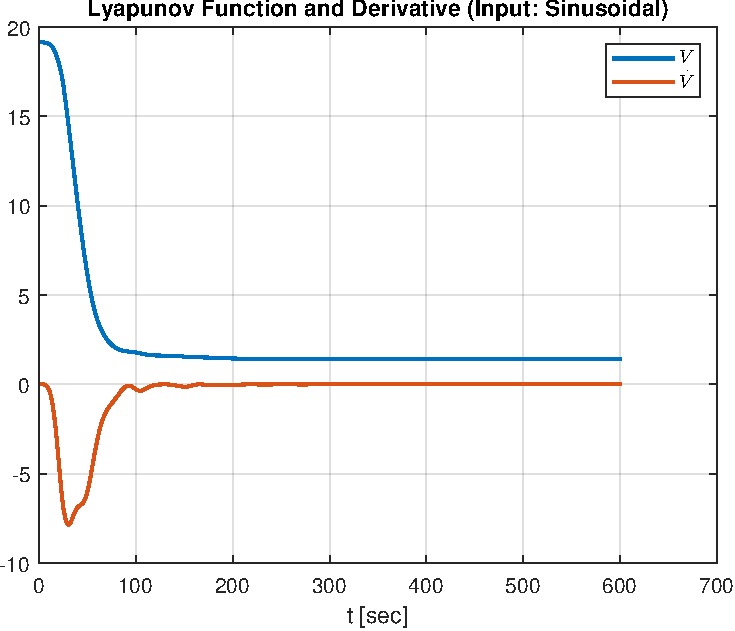
\includegraphics[width=\textwidth]{plot/task1_lyapunov_sinusoidal.pdf}
    \caption{}
    \label{fig:task1_lyapunov_sinusoidal}
  \end{subfigure}
  \caption{Γραφική παράσταση της συνάρτησης \selectlanguage{english}Lyapunov\selectlanguage{greek} καθώς και
  της παραγώγου της για α) βηματική είσοδο, β) $u(t) = 2 \sin t$}
  \label{fig:task1_lyapunov}
\end{figure}

Στο Σχήμα~\ref{fig:task1_identification_error_step} παρουσιάζεται το σφάλμα αναγνώρισης των δύο καταστάσεων 
για βηματική είσοδο, ενώ στο Σχήμα~\ref{fig:task1_identification_error_sinusoidal} απεικονίζεται το αντίστοιχο 
σφάλμα για είσοδο $u(t) = 2 \sin t$. Παρατηρούμε ότι και στις δύο περιπτώσεις τα σφάλματα συγκλίνουν στο μηδέν. 
Αυτό είναι αναμενόμενο, καθώς οι είσοδοι είναι φραγμένες και, σύμφωνα με το λήμμα 
\selectlanguage{english}Barbalat\selectlanguage{greek}, το σφάλμα αναγνώρισης τείνει στο μηδέν.

\begin{figure}
    \centering
    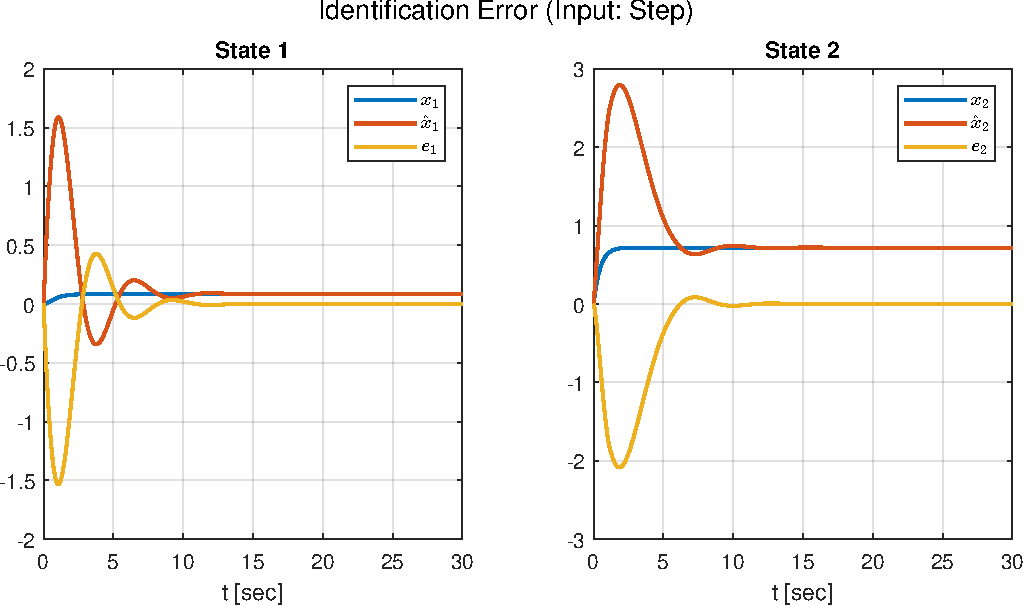
\includegraphics[width=1\linewidth]{plot/task1_identification_error_step.pdf}
    \caption{Σφάλμα αναγνώρισης για βηματική είσοδο}
    \label{fig:task1_identification_error_step}
\end{figure}

\begin{figure}
    \centering
    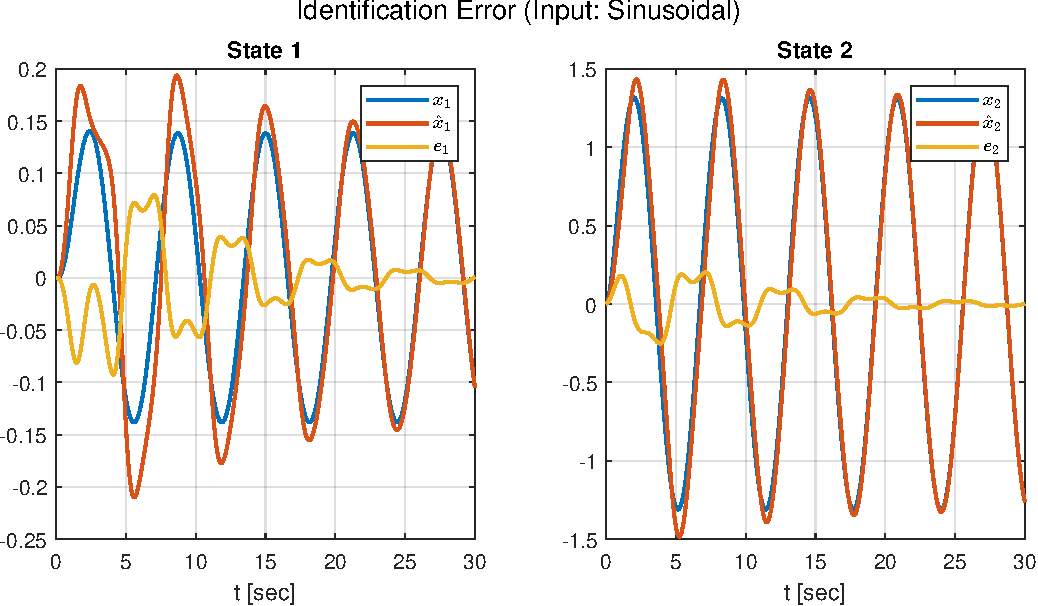
\includegraphics[width=1\linewidth]{plot/task1_identification_error_sinusoidal.pdf}
    \caption{Σφάλμα αναγνώρισης για είσοδο $u(t) = 2 \sin t$}
    \label{fig:task1_identification_error_sinusoidal}
\end{figure}

Στο Σχήμα~\ref{fig:task1_parameter_estimations} παρουσιάζονται οι εκτιμήσεις των παραμέτρων για βηματική είσοδο 
(αριστερά) και για ημιτονοειδή είσοδο $u(t) = 2 \sin t$ (δεξιά). Παρατηρούμε ότι και στις δύο περιπτώσεις 
ικανοποιούνται οι περιορισμοί $-3 \leq \hat{\alpha}_{11} \leq -1, \, b_2 \geq 1, \, \forall t$. 
Επιπλέον, για την ημιτονοειδή είσοδο όλες οι εκτιμήσεις συγκλίνουν στις πραγματικές τιμές των παραμέτρων, 
σε αντίθεση με την περίπτωση της βηματικής εισόδου. Αυτό οφείλεται στο γεγονός ότι η $u(t) = 2 \sin t$ 
ικανοποιεί τη ΣΕΔ, όπως αναλύθηκε προηγουμένως.

\begin{figure}[htbp]
  \centering
  \begin{subfigure}[b]{0.45\textwidth}
    \centering
    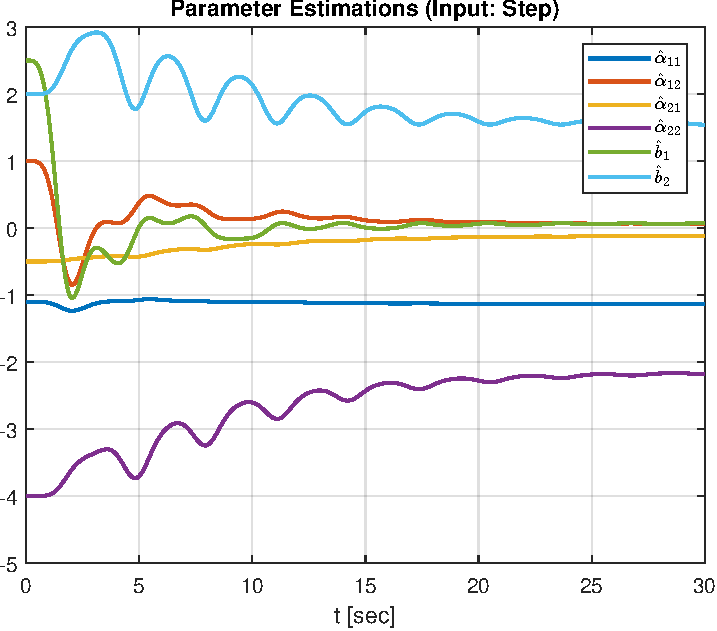
\includegraphics[width=\textwidth]{plot/task1_parameter_estimations_step.pdf}
    \caption{}
    \label{fig:task1_parameter_estimations_step}
  \end{subfigure}
  \hfill
  \begin{subfigure}[b]{0.45\textwidth}
    \centering
    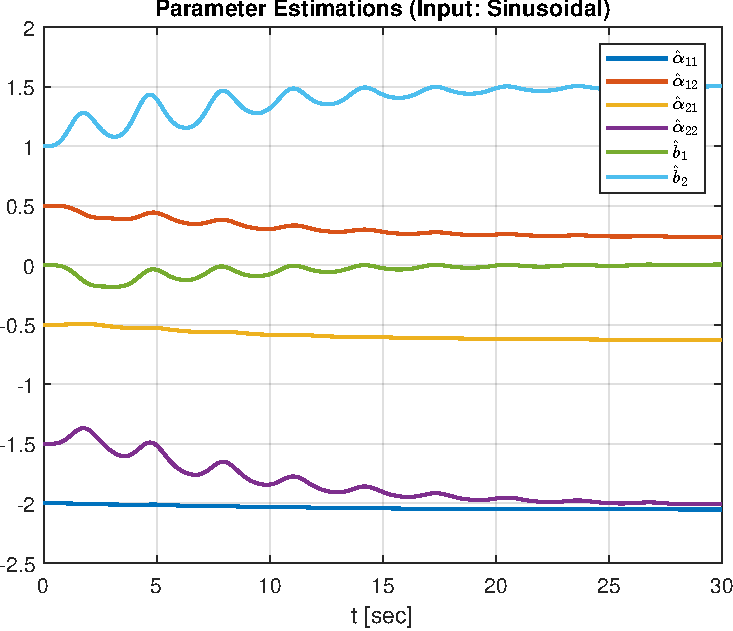
\includegraphics[width=\textwidth]{plot/task1_parameter_estimations_sinusoidal.pdf}
    \caption{}
    \label{fig:task1_parameter_estimations_sinusoidal}
  \end{subfigure}
  \caption{Εκτιμήσεις παραμέτρων για α) βηματική είσοδο, β) $u(t) = 2 \sin t$}
  \label{fig:task1_parameter_estimations}
\end{figure}


\subsection*{Εκτίμηση Παραμέτρων Παρουσία Σφάλματος Πόλωσης}
Θεωρούμε τώρα ότι στο σύστημά μας υπάρχει σφάλμα πόλωσης $\omega \in \mathbb{R}^2$ που να ικανοποιεί
$||\omega(t)|| \leq \bar{\omega}, \forall t \geq 0$, για κάποια άγνωστη σταθερά $\bar{\omega} > 0$.
Τα σφάλματα πόλωσης αποτελούν σταθερές ή αργά μεταβαλλόμενες διαταραχές που οφείλονται στην εσφαλμένη 
επιλογή της δομής του μοντέλου. Στην παρακάτω ανάλυση το σφάλμα πόλωσης μοντελοποιείται ως:
\begin{equation}
    \omega(t) = 
    \begin{bmatrix}
        \omega_1(t) \\
        \omega_2(t)
    \end{bmatrix} = 
    \begin{bmatrix}
        \bar{\omega} \sin(2 \pi f_w t) \\
        \bar{\omega} \cos(2 \pi f_w t)
    \end{bmatrix}, \quad t \geq 0
    \label{eq:bias_error}
\end{equation}
όπου $f_w << f_n$ με $f_n = \frac{\omega_n}{2 \pi}$ τη φυσική συχνότητα του συστήματος.

Παρουσία σφάλματος πόλωσης, οι κλασικές μέθοδοι εκτίμησης παραμέτρων πραγματικού χρόνου διασφαλίζουν ότι 
το σφάλμα αναγνώρισης $e$ παραμένει φραγμένο, δηλαδή $||e|| \leq \bar{\omega}$. Ωστόσο, η εκτίμηση των
παραμέτρων $\hat{\theta}$ ενδέχεται να αποκλίνει σημαντικά από τις πραγματικές τιμές $\theta^*$, 
οδηγώντας σε παραμετρικό σφάλμα $||\tilde{\theta}|| = ||\hat{\theta} - \theta|| \to \infty$.

Ένας τρόπος αντιμετώπισης της απόκλισης αυτής είναι η χρήση της μεθόδου προβολής, η οποία περιορίζει το 
διάνυσμα εκτίμησης εντός ενός κυρτού συνόλου $\Theta$, υπό την προϋπόθεση ότι $\theta^* \in \Theta$. 
Με αυτόν τον τρόπο διασφαλίζεται ότι $\hat{\theta} \in \Theta, \forall t \ge 0$, αποφεύγοντας την περίπτωση 
όπου $\hat{\theta} \to \infty$ δηλαδή την \textit{παραμετρική ολίσθηση}.

Αντί της μεθόδου προβολής, θα χρησιμοποιήσουμε έναν εύρωστο αλγόριθμο εκτίμησης παραμέτρων: 
τη μέθοδο κλίσης με διακοπτική $\sigma$-τροποποίηση.

\subsubsection*{Mέθοδος κλίσης με διακοπτική $\sigma$-τροποποίηση}

Θα φέρουμε το σύστημα της σχέσης (\ref{eq:state_space_form}) στην ισοδύναμη γραμμική παραμετροποιήσιμη 
μορφή. Από την πρώτη εξίσωση κατάστασης έχουμε:
\begin{equation}
    \dot{x}_1 = \alpha_{11} x_1 + \alpha_{12} x_2 + b_1 u
    \label{eq:linearly_parametrized_form_1}
\end{equation}
Εφόσον το $\dot{x}_1$ δεν είναι μετρήσιμο, χρησιμοποιούμε την προσέγγιση $\dot{x}_1 = s x_1$, οπότε η
(\ref{eq:linearly_parametrized_form_1}) γίνεται:
\begin{equation}
    \begin{aligned}
        &s x_1 = \alpha_{11} x_1 + \alpha_{12} x_2 + b_1 u \Rightarrow \\ 
        &(s - \alpha_{11}) x_1 = \alpha_{12} x_2 + b_1 u
    \end{aligned}
    \label{eq:linearly_parametrized_form_2}
\end{equation}
Φιλτράροντας τα δύο μέλη της (\ref{eq:linearly_parametrized_form_2}) με ευσταθές φίλτρο 1ης τάξης
$\Lambda(s) = s + \lambda, \, \lambda > 0$ παίρνουμε:
\begin{equation*}
    \begin{aligned}
        &\frac{s - \alpha_{11}}{\Lambda(s)} x_1 = \alpha_{12} \frac{x_2}{\Lambda(s)} + 
        b_1 \frac{u}{\Lambda(s)} \Rightarrow \\
        &\frac{\Lambda(s) - \lambda - \alpha_{11}}{\Lambda(s)} x_1 = \alpha_{12} \frac{x_2}{\Lambda(s)} + 
        b_1 \frac{u}{\Lambda(s)} \Rightarrow \\
        &\left(1 - \frac{\lambda + \alpha_{11}}{\Lambda(s)}\right) x_1 = \alpha_{12} \frac{x_2}{\Lambda(s)} + 
        b_1 \frac{u}{\Lambda(s)} \Rightarrow \\
        &x_1 = (\lambda + \alpha_{11})\frac{x_1}{\Lambda(s)} + \alpha_{12} \frac{x_2}{\Lambda(s)} + 
        b_1 \frac{u}{\Lambda(s)} \Rightarrow \\
        x_1 &=
        \begin{bmatrix}
            \lambda + \alpha_{11} & \alpha_{12} & b_1
        \end{bmatrix} \cdot
        \begin{bmatrix}
            \frac{x_1}{\Lambda(s)} & \frac{x_2}{\Lambda(s)} & \frac{u}{\Lambda(s)}
        \end{bmatrix}^{\top} \Rightarrow \\
        x_1 &= {\theta_1^*}^{\top} \phi
    \end{aligned} 
\end{equation*}
όπου
\begin{equation}
    \phi = 
    \begin{bmatrix}
        \frac{x_1}{\Lambda(s)} & \frac{x_2}{\Lambda(s)} & \frac{u}{\Lambda(s)}
    \end{bmatrix}^{\top}
    \label{eq:regresson_vector}
\end{equation}
το μετρήσιμο διάνυσμα οπισθοδρόμησης και
\begin{equation}
    \theta_1^* = 
    \begin{bmatrix}
        \lambda + \alpha_{11} & \alpha_{12} & b_1
    \end{bmatrix}^{\top}
    \label{eq:theta_star_1}
\end{equation}
το άγνωστο σταθερό διάνυσμα που εμπεριέχει τις πραγματικές τιμές των παραμέτρων προς εκτίμηση.

Εργαζόμενοι αντίστοιχα και για τη δεύτερη εξίσωση κατάστασης, καταλήγουμε στη γραμμικά 
παραμετροποιήσιμη μορφή:
\[
    x_2 = {\theta_2^*}^{\top} \phi
\]
με
\begin{equation}
    \theta_2^* = 
    \begin{bmatrix}
        \alpha_{21} & \lambda + \alpha_{22} & b_2
    \end{bmatrix}^{\top}
    \label{eq:theta_star_2}
\end{equation}

Οι εκτιμήσεις $\hat{\theta}_1, \, \hat{\theta}_2$ των $\theta_1^*, \, \theta_2^*$ της μεθόδου κλίσης με διακοπτική $\sigma$-τροποποίηση (στη συνεχή της μορφή) δίνονται από τη λύση του συστήματος:
\begin{equation}
    \begin{aligned}
    x_i &= {\theta_i^*}^{\top} \phi + \omega_i, \quad |\theta_i^*| \leq M \\
    \hat{x}_i &= \hat{\theta}_i \phi \\
    \dot{\hat{\theta}}_i &= - \gamma \sigma_{\delta}(\hat{\theta}_i) \hat{\theta}_i + 
    \gamma e_i \phi, \quad \gamma > 0 \\
    e_i &= x_i - \hat{x}_i
    \end{aligned}, \quad i = 1, 2
    \label{eq:gradient_switching_sigma_modification}
\end{equation}
όπου τα σφάλματα πόλωσης $\omega_i$ δίνονται από την (\ref{eq:bias_error}), $\hat{\theta}_i$ η εκτίμηση
του $\theta_i^*$, $M, \, \bar{\sigma}, \, \gamma > 0$ σχεδιαστικές σταθερές και
\begin{equation*}
    \sigma_{\delta}(\hat{\theta}) = 
    \left\{
    \begin{aligned}
        0&, \quad \texttt{αν } ||\hat{\theta}|| < M \\
        \bar{\sigma}\left(\frac{||\hat{\theta}||}{M} - 1\right)&, 
        \quad \texttt{αν } M \leq ||\hat{\theta}|| \leq 2M \\
        \bar{\sigma}&, \quad \texttt{αν } ||\hat{\theta}|| > 2M
    \end{aligned}, \quad \bar{\sigma} > 0
    \right.
\end{equation*}

Οι παράμετροι $M, \, \bar{\sigma}, \, \gamma > 0$ επιλέχθηκαν με τη μέθοδο
\selectlanguage{english}trial and error\selectlanguage{greek}.
Ειδικότερα, το $M$ επιλέγεται ώστε να ισχύει η απαίτηση $|\theta_i^*| \leq M$. Όσο πιο μεγάλο είναι το $M$,
τόσο ``καθιστερεί'' η εφαρμογή της $\sigma$-τρποποίησης, άρα τόσο επιτρέπεται στο $\hat{\theta}_i$ να ολισθήσει
σε μεγαλύτερες τιμές μέχρι να ``ενεργοποιηθεί'' η $\sigma$-τρποποίηση. Ο συντελεστής $\gamma$ ελέγχει την 
ταχύτητα σύγκλισης του $\hat{x}_i(t)$ στο $x_i(t)$. Αυξάνοντας την τιμή του $\gamma$ επιτυγχάνεται ταχύτερη
σύγκλιση. Πολύ μεγάλες τιμές του $\gamma$ όμως καθιστούν το σύστημά μας ``άκαμπτο''. Τέλος, η παράμετρος
$\bar{\sigma}$ ορίζει το πόσο βίαια ``τραβάει'' η μέθοδος τις εκτιμήσεις των παραμέτρων όταν απομακρύνονται 
από το κατώφλι $M$.



\end{document}
